
\begin{itemize}
	\item Initial ideas around technical challenges
	%(Possibly any initial ideas you have around solving some of the technical challenges)
	\begin{itemize}
		\item[] To start off, we would like to connect each screen being used to a terminal and connect all the terminals to a server(host) computer. We want to track the user's position and the direction the mobile device is pointing to, to be able to get the correct screen that the image is been "thrown" too. To get the user's position we will use 3 Bluetooth tags spread across a room and calculating the distance from each tag. To get the direction of the mobile device, we will use the built in compass of the mobile device.
	\end{itemize}
	
	\item Progress Reporting
	%(How you are going to keep the client informed about the status of your project)
	\begin{itemize}
		\item[] We will schedule regular meetings on a set interval (possibly two weeks) to ensure that we keep the momentum from the start of the project. This will create mini deadlines for us and thus we can achieve small victories throughout the development phase to ensure the project as a whole will succeed.
	\end{itemize}
	
	\item Development Methodology
	%(What development methodology you intend to follow)
	\begin{itemize}
	\item []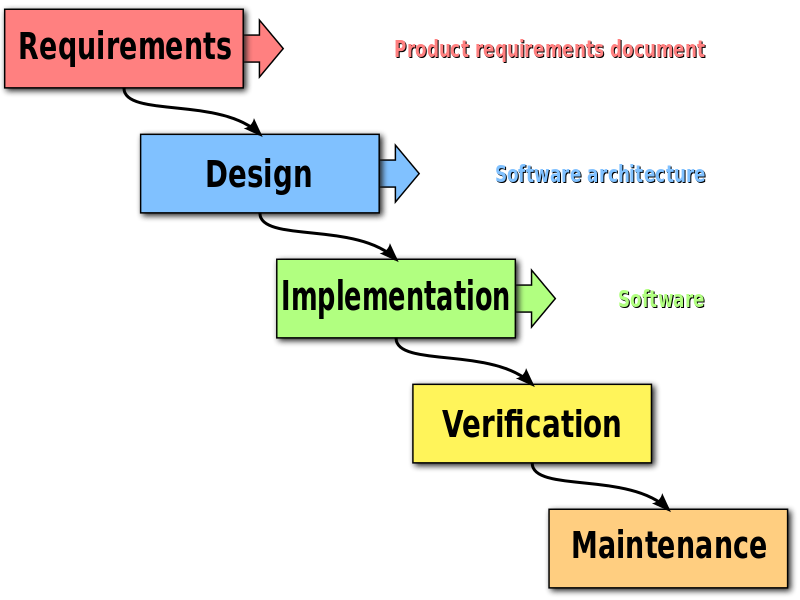
\includegraphics[scale=0.3]{./Images/Waterfall.png}
		\item[] We will use a sequential design process, used in software development processes, in which progress is seen as flowing steadily downwards through the phases of: 
		\begin{itemize}
			\item conception 
			\item initiation
			\item analysis
			\item design
			\item construction
			\item testing
			\item production/implementation
			\item maintenance
		\end{itemize}		 % Insert content here
		\item[] This is also known as the waterfall methodology.
	\end{itemize}
	
	\item Potential Technologies
	%(Potentially the technologies your team intends to use for the project (as far as these are not prescribed by the client))
	\begin{itemize}
		\item[] The technologies we plan to use are:
		\begin{itemize}
			\item On the Server
			\begin{itemize}
				\item NodeJS to connect to Bluetooth 4.0 device
			\end{itemize}
			\item On the Bluetooth tags
			\begin{itemize}
				\item Bluetooth 4.0 
			\end{itemize}
			\item On the Mobile Device
			\begin{itemize}
				\item Bluetooth 4.0
				
			\end{itemize}
		\end{itemize}
	\end{itemize}
	
	\item Outcome of the Project
	%(What the client will receive from you at the end of the project)
	\begin{itemize}
		\item The developed mobile application should include the following:
		\begin{itemize}
			\item[o] viewing images
			\item[o] Swipe image to load on screen being pointed to
			\item[o] Connecting to a server
			
		\end{itemize}
		
		\item The developed web server application should include the following:
		\begin{itemize}
			\item [o] User friendly GUI
			\item [o] The ability to view the current image "thrown" to the screen (Application)
			\item[o] Selecting Bluetooth tags near the server
		\end{itemize}
	\end{itemize}
	
\end{itemize}
